\documentclass[12pt, letterpaper]{article}
\usepackage{geometry}
\usepackage{hyperref}
\usepackage{times}
\usepackage{caption}
\usepackage{subcaption}
\usepackage{float}
\usepackage{graphicx}

\geometry{
  a4paper,
  margin=2.54cm
}

\title{Nonlocal means denoise}
\author{Alexander De Laurentiis}


\begin{document}

\maketitle
\pagebreak

\section{Motivations}
% What problem is, why wants to solve it.
Denoising images is a common need and has been done through averaging the pixels in the direct vicinity for the most part. Through doing so fine details are the image itself are often degraded or removed entirely. This caused the desire for a denoising algorithm that wouldn't alter the original image or remove details if possible. Therefore the NL-means algorithm wished to solve which of these in which it could.
\section{Approach}
\subsection{The Algorithm}
The NL-means operates by comparing the mean of the neighborhood of the current point $x$ with the gaussian neighborhoods of several other points in the image, and replacing the point $x$ with the most similiar neighborhood's The guassian kernel is used due to its relevance to denoising, and it is justified by normalizing it relative to the image to each point. 

\subsection{The Steps}
For every pixel i, the weighted average of all the pixels in the image will be calculated, this will be done as follows. For every other pixel j with respects to pixel i, the weight will be calculated. This weight will then be multiplied by the value of pixel j and summed for every j.

To compute the weights for each pixel j relative to i requires 3 primary parts. The first would be to find the euclidean distance betweem the vectors of the grey levels of the neighborhoods of each i and j, centered at i or j respectively and with $s\sigma^2$ added to the result.

Then the normalizing constant for the weight must be generated, $Z(i)$, which is denoted as $Z(i) = \sum_je^{-\frac{\|v(N_i)-v(N_j)\|_2^2,a}{h^2}}$ computed for every pixel j and summed. This constant is then divided into each weight's calculation. The weight is the gaussian of the pixel multiplied by the normalizing constant for j in the end.

\section{Results and critique}
Compared to other denoising algorithms the method noise extracted from the image shows very little structure. The algorithm may not perform noticibly better depending, but it is suited well for periodic or textured noise such as is present in CT scans. Its easier to find comparable locations for it when there are more open spaces. Therefore the algorthm as many has its uses and situations where it may outperform better than a local algorithm. It most importantly can denoise without reduction of details in the original image.


\centering
\section*{References}
\textbf{Non-local means image denoising}\\
A. Buades, B. Coll and J. -. Morel, "A non-local algorithm for image denoising," 2005 IEEE \textit{Computer Society Conference on Computer Vision and Pattern Recognition (CVPR'05)}, San Diego, CA, USA, 2005, pp. 60-65 vol. 2, doi: 10.1109/CVPR.2005.38.

\pagebreak
\centering
\section{Results}
\begin{figure}[H]
  \centering
  \begin{subfigure}[b]{.3\textwidth}
  
\includegraphics[width=\textwidth]{../imgs/stare}
  \caption{Original Image}
  \label{fig:5}
\end{subfigure}\\
  \begin{subfigure}[b]{.4\textwidth}
  \centering
  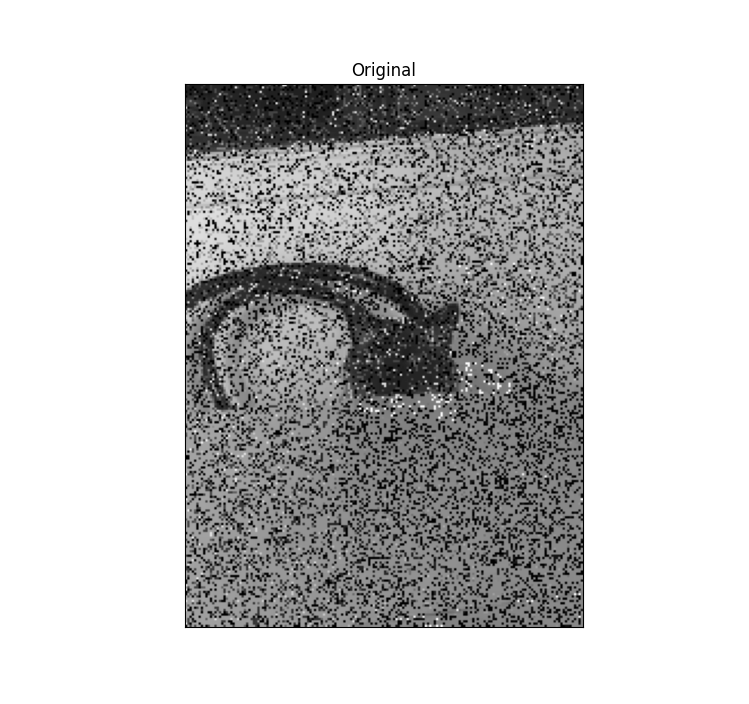
\includegraphics[width=\textwidth]{../imgs/original_stare_nl.png}
  \caption{greyscale plus noise}
  \label{fig:4}
\end{subfigure}
\begin{subfigure}[b]{.4\textwidth}
  \centering
  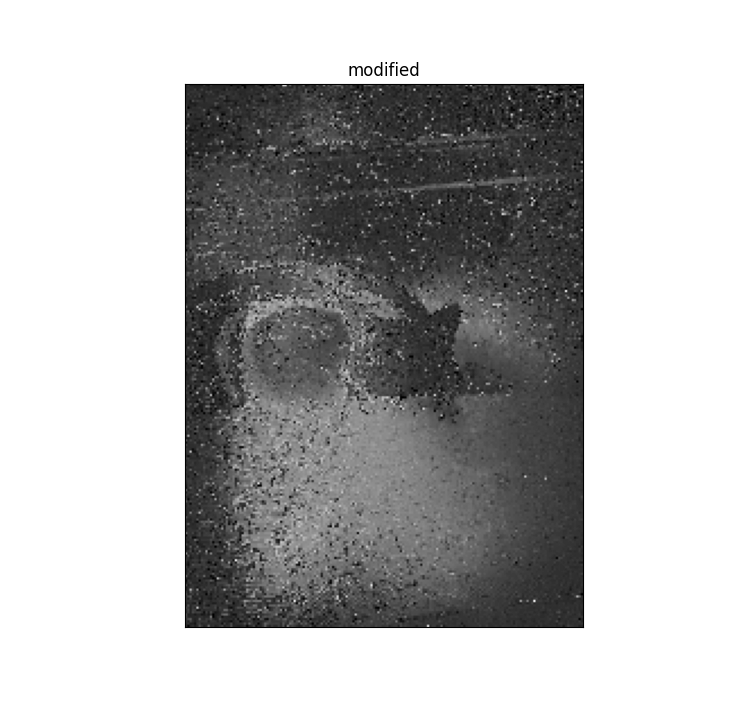
\includegraphics[width=\textwidth]{../imgs/filtered_stare_nl}
  \caption{Early Filtered result}
  \label{fig:4}
\end{subfigure}
\caption{Earlier iteration of the algorithm where it smoothed more than reduce the noise.}
\end{figure}

\end{document}